\documentclass[11pt]{amsart}
%prepared in AMSLaTeX, under LaTeX2e
\addtolength{\oddsidemargin}{-.7in}
\addtolength{\evensidemargin}{-.7in}
\addtolength{\topmargin}{-.6in}
\addtolength{\textwidth}{1.5in}
\addtolength{\textheight}{1.3in}
\newcommand{\normalspacing}{\renewcommand{\baselinestretch}{1.05}
        \tiny\normalsize}

\newtheorem*{thm}{Theorem}
\newtheorem*{defn}{Definition}
\newtheorem*{example}{Example}
\newtheorem*{problem}{Problem}
\newtheorem*{remark}{Remark}

\usepackage{amssymb,fancyvrb,alltt,xspace}
\usepackage{palatino}
\usepackage{fancyvrb}

\usepackage[final]{graphicx}
\usepackage{tikz}

\DefineVerbatimEnvironment{mVerb}{Verbatim}{numbersep=2mm,
frame=lines,framerule=0.1mm,framesep=2mm,xleftmargin=4mm,fontsize=\small}

% macros
\newcommand{\bb}{\mathbf{b}}
\newcommand{\bv}{\mathbf{v}}
\newcommand{\bx}{\mathbf{x}}
\newcommand{\by}{\mathbf{y}}

\newcommand{\CC}{\mathbb{C}}
\newcommand{\Div}{\nabla\cdot}
\newcommand{\eps}{\epsilon}
\newcommand{\grad}{\nabla}
\newcommand{\ZZ}{\mathbb{Z}}
\newcommand{\ip}[2]{\ensuremath{\left<#1,#2\right>}}
\newcommand{\lam}{\lambda}
\newcommand{\lap}{\triangle}
\newcommand{\RR}{\mathbb{R}}

\newcommand{\prob}[1]{\bigskip\noindent\large\textbf{#1}.\,\normalsize }
\newcommand{\ppart}[1]{\textbf{(#1)}\,\, }
\newcommand{\epart}[1]{\medskip\noindent\textbf{(#1)}\,\, }

\newcommand{\pts}[1]{\scriptsize [#1 points] \normalsize}
%\newcommand{\pts}[1]{}

\newcommand{\Matlab}{\textsc{Matlab}\xspace}
\newcommand{\Octave}{\textsc{Octave}\xspace}
\newcommand{\MO}{\Matlab/\Octave}


\begin{document}
\hfill \Large Name:\underline{\phantom{Ed Bueler really really long long long name}}
\medskip

\scriptsize \noindent Math 310 Numerical Analysis (Bueler) \hfill 10 December 2019
\medskip

\Large\centerline{\textbf{Final Exam}}

\smallskip
\large
\begin{center}
\textbf{In class.  No book or electronics.  1/2 sheet of notes allowed.}

\textbf{120 minutes maximum.  165 points total.}
\end{center}

\bigskip
\thispagestyle{empty}
\normalspacing

\prob{1}  \ppart{a}  \pts{5}  A differentiable function $f(x)$ and an iterate $x_k$ are shown on the axes below.  Sketch, with appropriate labeling, how \textbf{Newton's method} determines the next iterate $x_{k+1}$.

\begin{center}
\begin{tikzpicture}[scale=3.1]
\draw[->,gray,thin] (-2.0,0.0) -- (2.5,0.0) node[below] {$x$};
\draw[->,gray,thin] (0.0,-0.5) -- (0.0,1.2) node[left] {$y$};
\node[gray,xshift=-0.2cm,yshift=-0.2cm] at (0.0,0.0) {$0$};

\draw[domain=-1.8:2.4,smooth,variable=\x] plot ({\x},{0.4 +0.2*\x*\x*\x - 0.2*\x*\x - 0.5*\x)});

\draw (-0.5,-0.03) -- (-0.5,0.02);
\node at (-0.5,-0.1) {$x_k$};
\end{tikzpicture}
\end{center}

\medskip

\epart{b} \pts{5} Write \textbf{Newton's method} as a formula for determining the next iterate $x_{k+1}$ from the previous iterate $x_k$:

\qquad \Huge $\strut$ \large $x_{k+1}=$ \hspace{70mm}
\vfill

\epart{c} \pts{5} Write the \textbf{secant method} as a formula for determining the next iterate $x_{k+1}$ from the previous two iterates $x_k$ and $x_{k-1}$:

\qquad \Huge $\strut$ \large $x_{k+1}=$ \hspace{70mm}
\vfill


\newpage
\prob{2} \ppart{a} \pts{10} State \textbf{Taylor's theorem with remainder}.  \emph{Carefully state the hypotheses \emph{and} the conclusion of the theorem.}
\vfill

\epart{b} \pts{10}  Assume that the basepoint is $a=1$ and that the function is $f(x)=\cos(x/3)$.  How close is the degree 4 Taylor polynomial $P_4(x)$ to the function $f(x)$ on the interval $[0,2]$?  (\emph{Note that you are not asked to compute} $P_4(x)$; \emph{no points will be given for that.})  Answer by completing the following with a concrete upper bound.  (\emph{You may leave your concrete expression unsimplified.})

\bigskip
   $$|f(x) - P_4(x)| \le \hspace{5.0in}$$
\vfill


\newpage
\prob{3} \pts{15}  Table 10.3, printed on the last page, includes the order of accuracy $O(h^2)$ for the \textbf{composite trapezoid rule}.  However, we proved that if $f \in C^2[a,b]$, and if $h=(b-a)/n$ and $x_i = a+ih$ for $i=0,1,\dots,n$, then there is $\xi \in [a,b]$ so that
	$$\int_a^b f(x)\,dx = \frac{h}{2} \left[f(x_0) + 2 f(x_1) + 2 f(x_2) + \dots + 2 f(x_{n-1}) + f(x_n)\right] - \frac{1}{12} (b-a) h^2 f''(\xi).$$
Suppose we want to use this rule to compute $\int_0^1 e^{-x^2}\,dx$ to an accuracy of $10^{-8}$.  What $n$ is needed?  (\emph{Note you are not asked to apply the rule.  You may leave your concrete expression for $n$ unsimplified.})
\vfill

\prob{4} \pts{10}  Write two to four complete sentences to explain the ideas of \textbf{Clenshaw-Curtis quadrature (integration)} on the interval $[-1,1]$.  (\emph{Hint.  The ideas are not that different from those of the Newton-Cotes formulas.  Restate the basic ideas and then state the new ones, including a formula.})
\vspace{3.0in}


\newpage
\prob{5} \ppart{a} \pts{10}   Suppose $f(x) = e^x$.  Completely set up, \emph{but do not solve}, the \textbf{Vandermonde} linear system to find the degree 2 polynomial $p(x)=c_0+c_1x+c_2x^2$ which interpolates $f(x)$ at the points $x_0=-1,x_1=0,x_2=1$.
\vfill

\epart{b} \pts{10}  For the same $f(x)$ and interpolation points as in part \textbf{(a)}, write down \textbf{Lagrange's form} of the polynomial $p(x)$.   (\emph{Do not simplify.})
\vfill


\newpage
\prob{6} An actual proposed 8 bit version of the IEEE 754 standard for floating point representations, called \emph{minifloat}, has this set up:

\medskip\large
\begin{center}
\begin{tabular}{|c|c|c|c|c|c|c|c|c|} \hline
$s$ & $e_1$ & $e_2$ & $e_3$ & $e_4$ & $b_1$ & $b_2$ & $b_3$ \\ \hline
\end{tabular}
\end{center}
\medskip\normalsize

\noindent representing the number
\medskip\large
	$$x = (-1)^s\,(1.b_1 b_2 b_3)_2 \,\, 2^{(e_1 e_2 e_3 e_4)_2 + 2_{10}}$$
\normalsize

\noindent This scheme is designed to have the (surprising) property that all representable numbers are integers.  (\emph{The ``$+2_{10}$'' in the exponent is \emph{not} a misprint.})  Note the usual exception cases:
\begin{itemize}
\item exponent bits $(0000)_2$ define the number zero or subnormal numbers
\item exponent bits $(1111)_2$ define the other exceptions: $\pm\infty$ and NaN (\emph{\dots ignore the details})
\end{itemize}

\epart{a}  \pts{10}  What is the \textbf{largest number} that this system can represent?  (\emph{State the number in decimal notation and show the bits.  There is no need to simplify the number.})
\vfill

\epart{b}  \pts{10}  What is the \textbf{smallest \emph{normal} positive number} that this system can represent?  (\emph{State the number in decimal notation and show the bits. Please simplify the number.})
\vfill

\prob{Extra Credit}  \pts{3}  How do you represent 1 in the system?  What is the value of ``machine epsilon'' in this system?  Indeed, how do you define ``machine epsilon''?  Write complete sentences.  (\emph{Hint.  Think subnormal.})
\vfill


\newpage
\prob{7}  Consider the ODE IVP
	$$y' = t - 2y, \qquad y(0)=2.$$

\epart{a} \pts{10}  Do two steps of the Euler method with step size $h=\frac{1}{2}$.  This computes approximations of $y(0.5)$ and $y(1)$.
\vspace{3.0in}

\epart{b} \pts{10}  The trapezoid method, an implicit rule, is
    $$y_{k+1} = y_k + \frac{h}{2} \left(f(t_k,y_k) + f(t_{k+1},y_{k+1})\right).$$
Do two steps of this method, again with step size $h=\frac{1}{2}$.  This computes new approximations of $y(0.5)$ and $y(1)$.  (\emph{Hint. This requires easy algebra.})
\vfill

\newpage
\noindent \textbf{[continuation of problem 7]}

\medskip
\epart{c} \pts{5}  The exact solution to this ODE IVP is
    $$y(t)=\frac{t}{2} - \frac{1}{4} + \frac{9}{4} e^{-2t}.$$
Verify this.
\vspace{2.5in}

\epart{d} \pts{5}  The graph below already shows the exact solution.  Using the symbols shown in the legend, add your results from parts \textbf{(a)} and \textbf{(b)} to this graph.

\bigskip\bigskip
\begin{center}
\includegraphics[width=0.8\textwidth]{figs/eulertrapezoidgraph}
\end{center}


\newpage
\prob{8} \pts{15}  The midpoint method for the ODE IVP $y'=f(t,y)$, $y(t_0)=y_0$ is the pair of formulas
\begin{align*}
y_{k+1/2} &= y_k + \frac{h}{2} f(t_k,y_k) \\
y_{k+1} &= y_k + h f(t_{k+1/2},y_{k+1/2})
\end{align*}
Write a \Matlab algorithm which does $n$ steps of the midpoint method to approximately solve the ODE IVP on the interval $t_0 \le t \le t_f$.

\emph{Note that the time interval is described by a pair of numbers} \texttt{tspan = [t0 tf]} \emph{and that} $h=(t_f-t_0)/n$.  \emph{You may assume that the ODE is scalar, so $y_k$ in the above formulas is a single number, not a column vector.  Also, the returned variables should be suitable for plotting with} \texttt{plot(tt,yy)}. \emph{Finally, do not worry about adding comments.}

\medskip
\begin{mVerb}
function [tt,yy] = midpoint(f,tspan,y0,n)
































\end{mVerb}
\vfill

\newpage
\prob{10}  \pts{10}  Solve the following system of linear equations by Gauss elimination with partial pivoting and back substitution.  Show your steps, that is, indicate your row operations.

\begin{align*}
  x_1 +   x_2 &= 3 \hspace{4.0in} \\
4 x_1 - 3 x_2 &= -2.
\end{align*}
\vfill


\prob{11} \pts{10}  Suppose you have $n$ linear equations in $n$ unknowns,
    $$A\bx = \bb.$$
The algorithm used to solve such linear systems has two stages:
\begin{enumerate}
\item Gauss elimination with partial pivoting, and
\item back substitution.
\end{enumerate}
Approximately how many floating-point operations occur in these stages?  Which stage is more costly?  Answer quantitatively in a complete sentence or two.  (\emph{You do not need to count operations exactly, or prove your claims either.})
\vspace{2.5in}


\newpage
\begin{center}
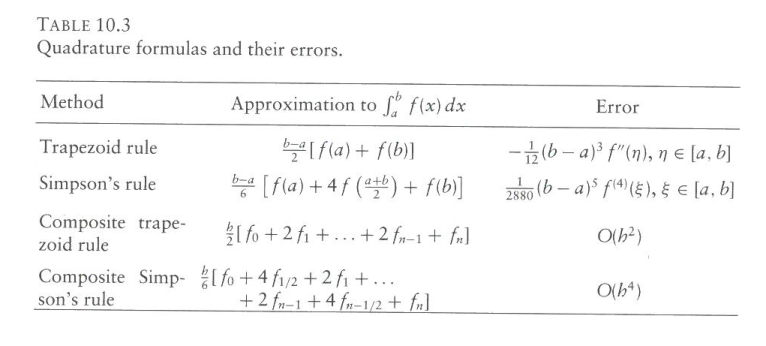
\includegraphics[width=0.95\textwidth]{figs/inttable}
\bigskip

%\noindent \hrulefill

[BLANK SPACE FOR SCRATCH WORK]
\end{center}
\thispagestyle{empty}
\vfill

\end{document}
